

\documentclass[10pt,twocolumn,letterpaper]{article}

%%%%%%%%% PAPER TYPE  - PLEASE UPDATE FOR FINAL VERSION
% \usepackage[review]{cvpr}      % To produce the REVIEW version
\usepackage{cvpr}              % To produce the CAMERA-READY version
%\usepackage[pagenumbers]{cvpr} % To force page numbers, e.g. for an arXiv version

% Include other packages here, before hyperref.
\usepackage{graphicx}
\usepackage{amsmath}
\usepackage{amssymb}
\usepackage{booktabs}
\usepackage[shortlabels]{enumitem}


% It is strongly recommended to use hyperref, especially for the review version.
% hyperref with option pagebackref eases the reviewers' job.
% Please disable hyperref *only* if you encounter grave issues, e.g. with the
% file validation for the camera-ready version.
%
% If you comment hyperref and then uncomment it, you should delete
% ReviewTempalte.aux before re-running LaTeX.
% (Or just hit 'q' on the first LaTeX run, let it finish, and you
%  should be clear).
\usepackage[pagebackref,breaklinks,colorlinks]{hyperref}


% Support for easy cross-referencing
\usepackage[capitalize]{cleveref}
\crefname{section}{Sec.}{Secs.}
\Crefname{section}{Section}{Sections}
\Crefname{table}{Table}{Tables}
\crefname{table}{Tab.}{Tabs.}


%%%%%%%%% PAPER ID  - PLEASE UPDATE
\def\cvprPaperID{*****} % *** Enter the CVPR Paper ID here
\def\confName{CVPR}
\def\confYear{2023}


\begin{document}
	
	%%%%%%%%% TITLE - PLEASE UPDATE
	\title{NTIRE 2023 Efficient SR Challenge Factsheet\\GateFormer is  What You Need for SR}
	
	\author{Yulong Liu, Jinpeng Shi, Shizhuang Weng\\
	Anhui university\\
	Anhui,China\\
	{\tt\small yl.liu88@outlook.com,jinpeeeng.s@gmail.com}
		% For a paper whose authors are all at the same institution,
		% omit the following lines up until the closing ``}''.
	% Additional authors and addresses can be added with ``\and'',
	% just like the second author.
	% To save space, use either the email address or home page, not both
}
\maketitle


\begin{figure*}[tph]
	\centering
	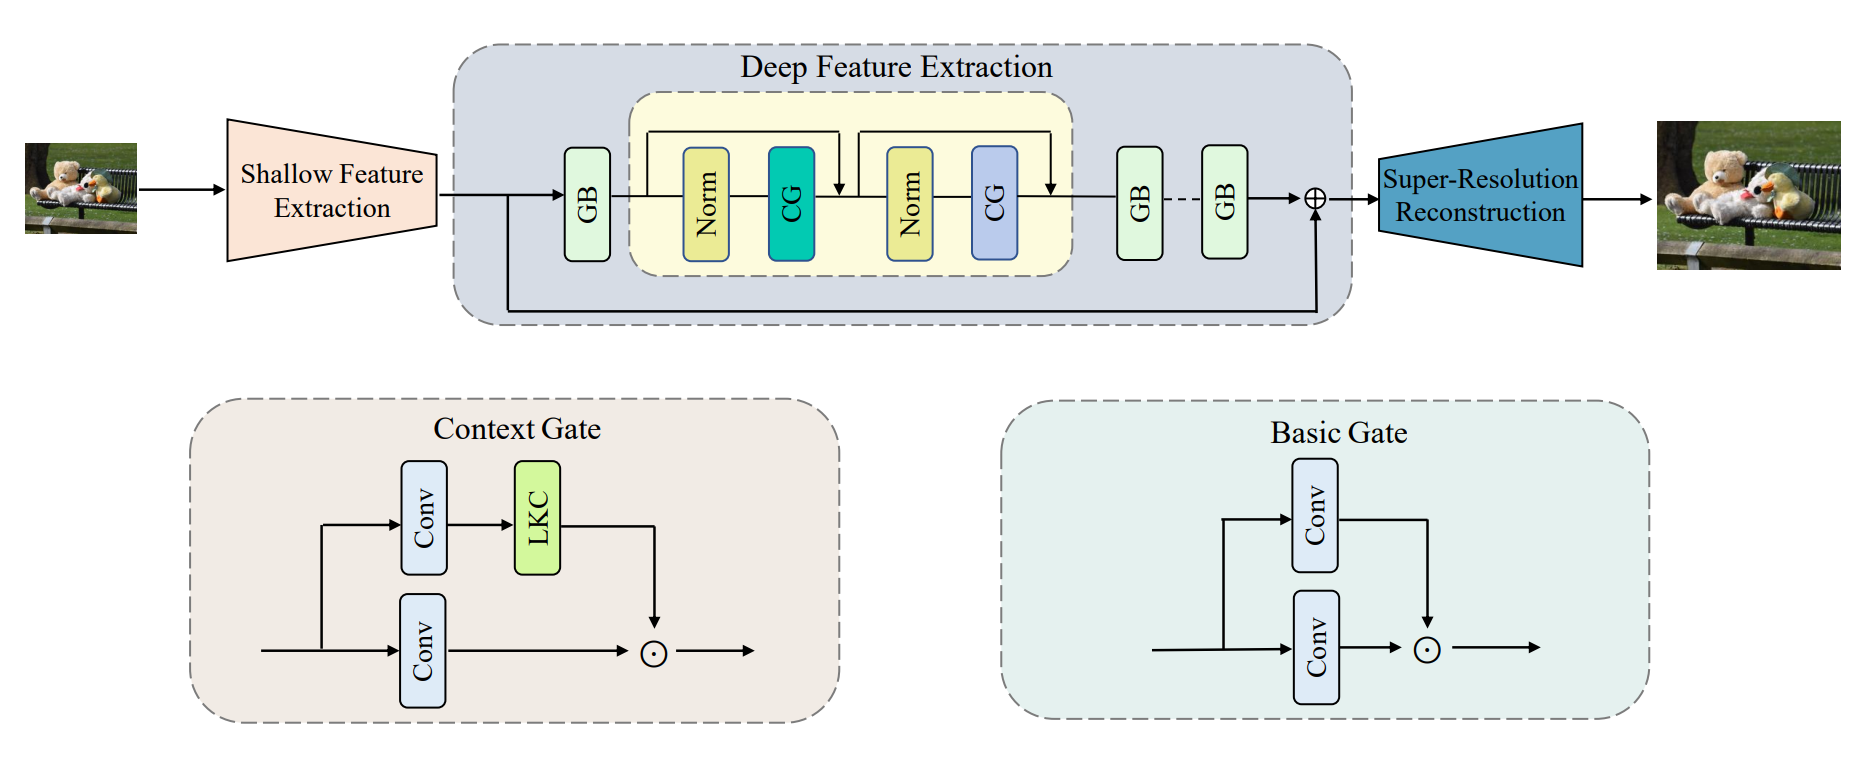
\includegraphics[width=1\linewidth]{Image/arch}
	\caption{Illustration of the GateFormer.}
	\label{arch}
\end{figure*}



\section{Team details}
\newcommand{\github}[1]{\href{https://github.com/#1/}{github.com/#1}}

\begin{itemize}
	\item Team name: \textbf{FRL Team 04}                                    
	\item Team leader name: \textbf{Yulong Liu}                               
	\item Team leader address, phone number, and email:
	\begin{itemize}
		\item address: \textbf{Anhui University, Hefei, China}
		\item phone number: \textbf{+86 183 5603 9028}
		\item email: \textbf{yl.liu88@outlook.com}
	\end{itemize}
	\item Rest of the team members: \textbf{Jinpeng Shi (advisor)}                   
	\item Team website URL (if any): \\ \github{Fried-Rice-Lab/FriedRiceLab}                               
	\item Affiliation: \textbf{Anhui University}
	\item Affiliation of the team and/or team members with NTIRE 2023 sponsors (check the workshop website): \textbf{N/A}
	\item User names and entries on the NTIRE 2023 Codalab competitions (development/validation and testing phases)    \begin{itemize}
		\item user name: \textbf{ylliu}
		\item development entries: \textbf{4}
		\item validation entries: \textbf{1}
	\end{itemize}
	\item Best scoring entries of the team during development/validation phase:
	\begin{table}[h]
		\centering
		\resizebox{\linewidth}{!}{
			\begin{tabular}{|c|c|c|c|c|}
				\hline
				PSNR&SSIM&Runtime&Params&Extra Data\\
				29.01 (13) 
				&0.83 (12)& 0.07 (22)& 199922.00 (17) &1.00 (1)\\
				\hline
			\end{tabular}
		}
	\end{table}
	\item Link to the codes/executables of the solution(s): \\ \github{LiuYLong/NTIRE2023\_ESR}
\end{itemize}



\section{Method details}
\subsection{Network Architecture}
Our team is committed to proposing a structurally simple and unified transformer to solve the single image super-resolution problems.The overall framework of the proposed GateFormer method is shown in the Figure \ref{arch}. A 3×3 convolutional layer is firstly used to extract shallow features from low-resolution images. Then multiple gate block modules are stacked to perform deep feature extraction on the shallow features. Finally the SR images are generated by upscaling module. Global skip connection is included to ensure better retention of useful information.


\subsection{Gate Block}
Inspired by Gated Linear Units\cite{chen2022simple}, we use two alternating gate modules to achieve this unified structure. One Basic Gate (BG) is used to replace the multi-layer perceptron (MLP)\cite{touvron2022resmlp} in the transformer. We also found that large convolution kernels can better capture global information to some extent. Therefore we upgraded the Basic Gate with a large convolution kernel as the Context Gate(CG) to replace the self-attention (SA)\cite{child2019generating,kitaev2020reformer} in the transformer.





\section{Training strategy}
We use DF2K (DIV2K\cite{agustsson2017ntire}, Flickr2K\cite{lim2017enhanced}) and LSDIR for datasets, and propose that the channel input is set to 37, the data augmentation method with $90^\circ$, $180^\circ$, $270^\circ$ random rotation and horizontal flip is used for training, the batchsize is set to 128, and the input patch size of LR is $64\times64$.Trained using Adam optimizer\cite{kingma2014adam} with $\beta_1$ = 0.9, $\beta_2$ = 0.999. The initialized learning rate is $5\times10^{-4}$ and decays to $1\times10^{-6}$ with the cosine learning rate. The model is optimized using the loss function of $L_1$ for a total of $1\times10^6$ iterations. 




\section{Experimental results}
We test our model on the DIV2K and LSDIR test sets, and the experiments are performed on a V100, using the official code. The results is shown in Table \ref{test}.
\begin{table}[h]
	\centering
	\resizebox{\linewidth}{!}{
		\begin{tabular}{|c|c|c|c|c|c|}
			\specialrule{0em}{1pt}{0pt}
			\hline
			PSNR&SSIM&Params[K]&FLOPs[G]&Conv&Average Runtime[ms]\\
			\hline
			27.03 (19)&0.81 (12)&199 (10)&12.75&100&0.05 (16)\\
			\hline
	\end{tabular}}
	\caption{ Result of DIV2K and LSDIR test sets}
	\label{test}
	
\end{table}







%%%%%%%%% REFERENCES
{\small
	\bibliographystyle{ieee_fullname}
	\bibliography{egbib}
}

\end{document}
